\newpage

\subsection{The Work Methodology and Auto-Evaluation}

\quad For this work, we used a work methodology where, during the various meetings we held, we usually divided them into 3 parts. The first part consisted of analyzing the results of each of the team members, in case there were tasks to be done for that meeting. The second part of the meeting consists of analyzing what needs to be done in general for the next delivery, in that same time we visualized and aligned all the tasks to be done for the next presentation. Finally, the third and final part of the meeting consisted of dividing these tasks previously defined by each of the elements of the group.\\

We usually have at least 2 meetings in the space from one class to another, but there were situations where more than one meeting was necessary in that space of time, mainly due to doubts in the execution of the tasks, in these situations we normally gathered everyone by video call and resolved let's get to the problem. \\

For the Auto-Evaluation our group thinks this the grade that each element of the group deserves:
\\
\begin{figure}[H]
    \centering
    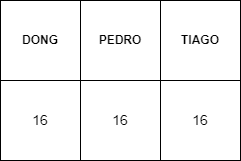
\includegraphics[width=0.4\textwidth]{assets/notas.png}
    \caption{Group Auto-Evaluation}
    \label{fig:notas}
    \end{figure}